%%%%%%%%%%%%%%%%%%%%%%%%%%%%%%%%%%%%%%%%%%%%%%
%
%		My Thesis
%
%		EDOC Template
%		2011
%
%%%%%%%%%%%%%%%%%%%%%%%%%%%%%%%%%%%%%%%%%%%%%%


%%%%%%%%%%%%%%%%%%%%%%%%%%%%%%%%%%%%%%%%%%%%%%
%
%		Thesis Settings
%
%		EDOC Template
%		2011
%
%%%%%%%%%%%%%%%%%%%%%%%%%%%%%%%%%%%%%%%%%%%%%%
\documentclass[a4paper,12pt,fleqn,print,oneside]{book}

\usepackage[T1]{fontenc}
\usepackage[utf8]{inputenc}
\usepackage[english, vietnamese]{babel}
%\usepackage{bookman}

%%%%%%%%%%%%%%%%%%%%%%%%%%%%%%%%%%%%%%%%%%%%%%%
%% EDOC THESIS TEMPLATE: Variant 1.0 -> Latin modern, large text width&height
%%%%%%%%%%%%%%%%%%%%%%%%%%%%%%%%%%%%%%%%%%%%%%%
%\usepackage{lmodern}
%\usepackage[a4paper,top=22mm,bottom=28mm,inner=35mm,outer=25mm]{geometry}
%%%%%%%%%%%%%%%%%%%%%%%%%%%%%%%%%%%%%%%%%%%%%%%

%%%%%%%%%%%%%%%%%%%%%%%%%%%%%%%%%%%%%%%%%%%%%%
% EDOC THESIS TEMPLATE: Variant 2.0 -> Utopia, Gabarrit A (lighter pages)
%%%%%%%%%%%%%%%%%%%%%%%%%%%%%%%%%%%%%%%%%%%%%%
%\usepackage[libertine,cmintegrals,cmbraces,vvarbb]{newtxmath}
\usepackage{mathpazo}
%\usepackage{utopia} % Utopia font-typesetting including mathematical formula compatible with newer TeX-Distributions (>2010)
%\usepackage{pia} % on older systems -> use this package instead of fourier in combination with mathdesign for better looking results
%\usepackage[adobe-utopia]{mathdesign}
\setlength{\textwidth}{146.8mm} % = 210mm - 37mm - 26.2mm
\setlength{\oddsidemargin}{11.6mm} % 37mm - 1in (from hoffset)
\setlength{\evensidemargin}{0.8mm} % = 26.2mm - 1in (from hoffset)
\setlength{\topmargin}{-2.2mm} % = 0mm -1in + 23.2mm 
\setlength{\textheight}{221.9mm} % = 297mm -29.5mm -31.6mm - 14mm (12 to accomodate footline with pagenumber)
\setlength{\headheight}{14pt}
%%%%%%%%%%%%%%%%%%%%%%%%%%%%%%%%%%%%%%%%%%%%%%


\usepackage[T1]{fontenc}
\usepackage{lmodern}
%\setlength{\parindent}{0pt}

\usepackage{setspace} % increase interline spacing slightly
\setstretch{1.1}

\makeatletter
\setlength{\@fptop}{0pt}  % for aligning all floating figures/tables etc... to the top margin
\makeatother


\usepackage{graphicx,xcolor}
\graphicspath{{images/}}

%\usepackage{subfig}
\usepackage{booktabs}
\usepackage{lipsum}
\usepackage{microtype}
\usepackage{url}
\usepackage[final]{pdfpages}

\usepackage{fancyhdr}
\renewcommand{\sectionmark}[1]{\markright{\thesection\ #1}}
\pagestyle{fancy}
	\fancyhf{}
	\renewcommand{\headrulewidth}{0.4pt}
	\renewcommand{\footrulewidth}{0pt}
	\fancyhead[OR]{\bfseries \nouppercase{\rightmark}}
	\fancyhead[EL]{\bfseries \nouppercase{\leftmark}}
	\fancyfoot[EL,OR]{\thepage}
\fancypagestyle{plain}{
	\fancyhf{}
	\renewcommand{\headrulewidth}{0pt}
	\renewcommand{\footrulewidth}{0pt}
	\fancyfoot[EL,OR]{\thepage}}
\fancypagestyle{addpagenumbersforpdfimports}{
	\fancyhead{}
	\renewcommand{\headrulewidth}{0pt}
	\fancyfoot{}
	\fancyfoot[RO,LE]{\thepage}
}

\usepackage{listings}
\lstset{language=[LaTeX]Tex,tabsize=4, basicstyle=\scriptsize\ttfamily, showstringspaces=false, numbers=left, numberstyle=\tiny, numbersep=10pt, breaklines=true, breakautoindent=true, breakindent=6pt}

\usepackage{hyperref}
\hypersetup{pdfborder={0 0 0},
	colorlinks=true,
	linkcolor=black,
	citecolor=black,
	urlcolor=black}
\urlstyle{same}

\makeatletter
\def\cleardoublepage{\clearpage\if@twoside \ifodd\c@page\else
    \hbox{}
    \thispagestyle{empty}
    \newpage
    \if@twocolumn\hbox{}\newpage\fi\fi\fi}
\makeatother \clearpage{\pagestyle{plain}\cleardoublepage}


%%%%% CHAPTER HEADER %%%%
\usepackage{color}
\usepackage{tikz}
\usepackage[explicit]{titlesec}
\newcommand*\chapterlabel{}
%\renewcommand{\thechapter}{\Roman{chapter}}
\titleformat{\chapter}[display]  % type (section,chapter,etc...) to vary,  shape (eg display-type)
	{\normalfont\bfseries\Huge} % format of the chapter
	{\gdef\chapterlabel{\thechapter\ }}     % the label 
 	{0pt} % separation between label and chapter-title
 	  {\begin{tikzpicture}[remember picture,overlay]
    \node[yshift=-8cm] at (current page.north west)
      {\begin{tikzpicture}[remember picture, overlay]
        \draw[fill=black] (0,0) rectangle(35.5mm,15mm);
        \node[anchor=north east,yshift=-7.2cm,xshift=34mm,minimum height=30mm,inner sep=0mm] at (current page.north west)
        {\parbox[top][30mm][t]{15mm}{\raggedleft $\phantom{\textrm{l}}$\color{white}\chapterlabel}};  %the black l is just to get better base-line alingement
        \node[anchor=north west,yshift=-7.2cm,xshift=37mm,text width=\textwidth,minimum height=30mm,inner sep=0mm] at (current page.north west)
              {\parbox[top][30mm][t]{\textwidth}{\color{black}#1}};
       \end{tikzpicture}
      };
   \end{tikzpicture}
   \gdef\chapterlabel{}
  } % code before the title body

\titlespacing*{\chapter}{0pt}{50pt}{30pt}
\titlespacing*{\section}{0pt}{12pt}{*0}  % 13.2pt is line spacing for a text with 11pt font size
\titlespacing*{\subsection}{0pt}{12pt}{*0}
\titlespacing*{\subsubsection}{0pt}{12pt}{*0}

\newcounter{myparts}
\newcommand*\partlabel{}
\titleformat{\part}[display]  % type (section,chapter,etc...) to vary,  shape (eg display-type)
	{\normalfont\bfseries\Huge} % format of the part
	{\gdef\partlabel{\thepart\ }}     % the label 
 	{0pt} % separation between label and part-title
 	  {\setlength{\unitlength}{20mm}
	  \addtocounter{myparts}{1}
	  \begin{tikzpicture}[remember picture,overlay]
    \node[anchor=north west,xshift=-65mm,yshift=-6.9cm-\value{myparts}*20mm] at (current page.north east) % for unknown reasons: 3mm missing -> 65 instead of 62
      {\begin{tikzpicture}[remember picture, overlay]
        \draw[fill=black] (0,0) rectangle(62mm,20mm);   % -\value{myparts}\unitlength
        \node[anchor=north west,yshift=-6.1cm-\value{myparts}*20mm,xshift=-60.5mm,minimum height=30mm,inner sep=0mm] at (current page.north east)
        {\parbox[top][30mm][t]{55mm}{\raggedright \color{white}Part \partlabel $\phantom{\textrm{l}}$}};  %the phantom l is just to get better base-line alingement
        \node[anchor=north east,yshift=-6.1cm-\value{myparts}*20mm,xshift=-63.5mm,text width=\textwidth,minimum height=30mm,inner sep=0mm] at (current page.north east)
              {\parbox[top][30mm][t]{\textwidth}{\raggedleft \color{black}#1}};
       \end{tikzpicture}
      };
   \end{tikzpicture}
   \gdef\partlabel{}
  } % code before the title body
 
 
\usepackage{lastpage}
 
%\fancyhead[R]{
%	\begin{tabular}{l}
%		\tiny \bf \\
%		\tiny \bf 
%	\end{tabular}  }

%\fancyfoot{} % clear all footer fields
%\fancyfoot[R]{\ttfamily {\thepage}}
%\fancyfoot[L]{\scriptsize \ttfamily LUẬN VĂN TỐT NGHIỆP - Niên khóa 2014-2018}
%\fancyfoot[R]{\scriptsize \ttfamily Trang {\thepage}/\pageref{LastPage}}
%\renewcommand{\headrulewidth}{0.3pt}
%\renewcommand{\footrulewidth}{0.3pt}

\usepackage{amsmath}
% Fix the problem with delimiter size caused by fourier and amsmath packages.
\makeatletter
\def\resetMathstrut@{%
  \setbox\z@\hbox{%
    \mathchardef\@tempa\mathcode`\(\relax
      \def\@tempb##1"##2##3{\the\textfont"##3\char"}%
      \expandafter\@tempb\meaning\@tempa \relax
  }%
  \ht\Mathstrutbox@1.2\ht\z@ \dp\Mathstrutbox@1.2\dp\z@
}
\makeatother


%%%%%%%%%%%%%%%%%%%%%%%%%%%%%%%%%%%%%%%%%%%%%%
%
%		Thesis Settings
%		Custom settings
%
%		2011
%
%%%%%%%%%%%%%%%%%%%%%%%%%%%%%%%%%%%%%%%%%%%%%%

%
%   Use this file for your own custom packages, command-definitions, etc...
%


% the following lines are for creating a simplified TO-DO box. However since boites is not per default installed with all latex-distributions, we have removed this example again
% if you want to use it and do not have "boites" installed, you can get it from here: http://www.ctan.org/tex-archive/macros/latex/contrib/boites
%
%\usepackage{boites,boites_exemples}
%\newcommand{\todolist}[1]{\begin{boiteepaisseavecuntitre}{TO DO in this chapter} #1 \end{boiteepaisseavecuntitre}}  % creates a little box
% %\newcommand{\todolist}[1]{}  % to be used when to do is not to be printed
\usepackage[numbers]{natbib}
\bibliographystyle{IEEEtranN}
\usepackage[noabbrev, nameinlink]{cleveref}
\usepackage{pdfpages}
\usepackage{enumitem}
\usepackage{textcomp}
\usepackage{pifont}
\usepackage{tabto}
\usepackage{amssymb}
\usepackage{hyperref}
\usepackage{booktabs}
\usepackage{graphicx}
\usepackage{array}
\usepackage{pdflscape}
%\usepackage{subcaption}
\usepackage{subfig}
\usepackage{forest}

\makeatletter
\renewcommand*\l@figure{\@dottedtocline{1}{1em}{3.2em}}
\makeatother
  % place your custom packages, etc... in this file!
%\input{thesis-info.tex}

%%%%%%%%%%%%%%%%%%%%%%%%%%%%%%%%%%%%%%%%%%%%%%
%%%%% HEAD: Book-Begin
%%%%%%%%%%%%%%%%%%%%%%%%%%%%%%%%%%%%%%%%%%%%%%
\begin{document}
\frontmatter
%\begin{titlepage}
%\begin{center}
%%\large
%\sffamily
%
%
%\null\vspace{2cm}
%{\huge A survey of various data dissemination schemes for Vehicular Ad-hoc NETwork} \\[24pt] 
%\textcolor{gray}{\small{THIS IS A TEMPORARY TITLE PAGE \\ It will be replaced for the final print by a version \\ provided by the service academique.}}
%    
%\vfill
%
%\begin{tabular} {cc}
%\parbox{0.3\textwidth}{\includegraphics[width=4cm]{images/epfl}}
%&
%\parbox{0.7\textwidth}{%
%	Thèse n. 1234 2011\\
%	présenté le 12 Mars 2011\\
%	à la Faculté des Sciences de Base\\
%	laboratoire SuperScience\\
%	programme doctoral en SuperScience\\
%%
%%	ÉCOLE POLYTECHNIQUE FÉDÉRALE DE LAUSANNE\\
%	École Polytechnique Fédérale de Lausanne\\[6pt]
%	pour l'obtention du grade de Docteur ès Sciences\\
%	par\\ [4pt]
%	\null \hspace{3em} Paolino Paperino\\[9pt]
%%
%\small
%acceptée sur proposition du jury:\\[4pt]
%%
%    Prof Name Surname, président du jury\\
%    Prof Name Surname, directeur de thèse\\
%    Prof Name Surname, rapporteur\\
%    Prof Name Surname, rapporteur\\
%    Prof Name Surname, rapporteur\\[12pt]
%%
%Lausanne, EPFL, 2011}
%\end{tabular}
%\end{center}
%\vspace{2cm}
%\end{titlepage}

\begin{titlepage}
	%
\includepdf{head/cover.pdf}
\thispagestyle{empty}
\begin{center}
	\begin{large}
		\textbf{Đại học Quốc gia Thành phố Hồ Chí Minh}
	\end{large} \\
	\begin{large}
		\textbf{Trường Đại học Bách Khoa}
	\end{large} \\
	\begin{large}
		\textbf{Khoa Khoa học và Kỹ thuật Máy tính}
	\end{large} \\
	\textbf{--------------------  *  ---------------------}\\[1.2cm]
	
	\begin{center}
		
\includegraphics[scale=.7]{images/HCMUT_official_logo.png}\\[1.0cm]
	\end{center}
	
	{\fontsize{23pt}{1}\selectfont \textbf{Luận Văn Tốt Nghiệp}}\\[1.5cm]
	
	{\fontsize{24pt}{1}\selectfont \textbf{Đề tài: Nhận dạng biển số xe trên nền tảng hệ thống vi mạch không đồng nhất} }\\[1.75cm]
\end{center}

\hspace{2cm} Hội đồng \hspace{72pt} :  \hspace{5pt} \textbf{\parbox[t]{10cm}{
		Kỹ Thuật Máy Tính
}} 

\hspace{2cm} Giáo viên hướng dẫn \hspace{15pt} :  \hspace{4pt} \textbf{\parbox[t]{8cm}{
		TS. Nguyễn Trần Hữu Nguyên
}} 

\hspace{2cm} Giáo viên phản biện \hspace{18pt} :  \hspace{4pt} \textbf{\parbox[t]{8cm}{
		TS. Phạm Quốc Cường
}} \\


\hspace{2cm} Sinh viên thực hiện \hspace{22pt} : \hspace{4pt}
\textbf{\parbox[t]{20cm}{
		Nguyễn Xuân Nam \hspace{15pt} - 1512098\\
}}


\vspace{1.5cm}
%	\vspace{1.75cm}
\begin{center}
	%{\fontsize{20pt}{1} TP Hồ Chí Minh}\\
	{\fontsize{20pt}{1} \today}
\end{center}

\end{titlepage}




\cleardoublepage
\thispagestyle{empty}


\vspace*{3cm}

\begin{raggedleft}
    	I think, therefore I am;\\
     --- René Descartes\\
\end{raggedleft}

\vspace{4cm}




\setcounter{page}{0}
\chapter*{Lời cam đoan}
\markboth{Lời cam đoan}{Lời cam đoan}
\addcontentsline{toc}{chapter}{Lời cam đoan}
\vspace{1.0cm}
Nhóm cam đoan mọi điều được ghi trong báo cáo, cũng như mã nguồn là do nhóm tự thực hiện - trừ các kiến thức tham khảo có trích dẫn cũng như mã nguồn mẫu do chính nhà sản xuất cung cấp, hoàn toàn không sao chép từ bất cứ nguồn nào khác. Nếu lời cam đoan trái với sự thật, nhóm xin chịu mọi trách nhiệm trước Khoa và Nhà trường.
\begin{flushright}
Nhóm sinh viên thực hiện đề tài 
\end{flushright}


\bigskip
 
%\noindent\textit{Lausanne, 12 Mars 2011}
%\hfill D.~K.

\chapter*{Lời cảm ơn}
\markboth{Lời cảm ơn}{Lời cảm ơn}
\addcontentsline{toc}{chapter}{Lời cảm ơn}
\onehalfspacing
\vspace{1.0cm}
Sau bốn năm theo học tại khoa Khoa học Kĩ thuật Máy tính trường Đại học Bách khoa TP. Hồ Chí Minh, em đã được áp dụng tất cả những kiến thức đã học để thực hiện luận văn tốt nghiệp, đề tài cuối cùng mang tính quyết định kết quả học tập và quá trình tốt nghiệp.\\

Em xin chân thành cảm ơn quý thầy cô trong Khoa đã mang đến những kiến thức bổ ích trong suốt quãng đời sinh viên, đặc biệt là thầy Phạm Hoàng Anh đã giúp đỡ em trong quá trình thực hiện cũng như quá trình hoàn thiện luận văn. Em cũng gửi lời cảm ơn đến một số bạn bè trong Khoa đã hỗ trợ giúp em tiết kiệm được thời gian tìm hiểu đề tài. \\

Em đã cố gắng hết sức để tránh các sai sót, nhưng nếu có phát hiện thì mong quý thầy cô góp ý để em càng hoàn thiện đề tài hơn. Cuối cùng em xin gửi lời chúc sức khỏe và cảm ơn chân thành nhất.
\begin{flushright}
 Nhóm sinh viên thực hiện đề tài 
\end{flushright}

\bigskip
 
%\noindent\textit{Lausanne, 12 Mars 2011}
%\hfill D.~K.

%\input{head/achievement}
% English abstract
\cleardoublepage
\chapter*{Tóm tắt}
%\markboth{Abstract}{Abstract}
\addcontentsline{toc}{chapter}{Tóm tắt} % adds an entry to the table of contents
\vspace{1.0cm}


\vskip0.5cm
%put your text here


%\endgroup			
%\vfill


\tableofcontents
\pdfbookmark{\contentsname}{Mục lục}
\cleardoublepage
\phantomsection
\addcontentsline{toc}{chapter}{Mục Lục Hình} % 
\addcontentsline{toc}{chapter}{Danh Sách Bảng} %
adds an entry to the table of contents
\listoffigures
\cleardoublepage
\phantomsection
%\addcontentsline{toc}{chapter}{List of tables} % adds an entry to the table of contents
%\listoftables
%\cleardoublepage
%\phantomsection
\newcommand{\abbrlabel}[1]{\makebox[3cm][l]{\textbf{#1}\ \dotfill}}
\newenvironment{abbreviations}{\begin{list}{}{\renewcommand{\makelabel}{\abbrlabel}}}{\end{list}}

\chapter*{Thuật ngữ \& từ viết tắt}
\thispagestyle{empty}
\pagestyle{empty}
\addcontentsline{toc}{chapter}{Thuật ngữ \& từ viết tắt}
\vspace{1.0cm}
\begin{abbreviations}
	\item .
\end{abbreviations}
% your list of symbols here, if needed.


% space before each new paragraph according to the template guidelines.
%(needs to be after titlepage and frontmatter to keep the table of contents lists short)
\setlength{\parskip}{1em}


%%%%%%%%%%%%%%%%%%%%%%%%%%%%%%%%%%%%%%%%%%%%%%
%%%%% MAIN: The chapters of the thesis
%%%%%%%%%%%%%%%%%%%%%%%%%%%%%%%%%%%%%%%%%%%%%%
\mainmatter
\chapter{Giới thiệu đề tài}
\pagestyle{fancy}
    \section{Giới thiệu}
    Với sự gia tăng nhanh chóng của số lượng phương tiện giao thông, con người ngày càng cần những hệ thống thông minh hơn cho việc quản lý hàng tá phương tiện giao thông này. Đóng một phần quan trọng trong hệ thống này đó là những ứng dụng liên quan đến nhận dạng biển số bởi tính thiết thực của chúng. Hiện đã có nhiều nghiên cứu cũng như áp dụng những hệ thống nhận dạng biển số trong việc quản lý bãi xe, phát hiện vi phạm giao thông, hệ thống thu phí tự động... Các hệ thống nhận dạng biển số thương mại nổi tiếng có thể kể đến là OPENALPR hay SIGHTHOUND.

    Hệ thống nhận dạng biển số gồm ba giai đoạn cơ bản nhất đó là: xác định vị trí của biển số, phân tách các kí tự trên biển số và nhận diện các kí tự đó. Trong đó, giai đoạn đầu tiên giữ vai trò vô cùng quan trọng. Nó cần độ chính xác rât cao thậm chí là hoàn hảo bởi việc xác định sai vị trí của biển số sẽ dẫn đến hậu quả cho những giai đoạn tiếp theo. Nhiều giải pháp đã được áp dụng cho giai đoạn này (sử dụng xử lý ảnh hay áp dụng những giải thuật học máy,...) nhằm giảm thời gian xử lí cũng như giảm tỉ lệ lỗi.

    Với xử lí ảnh, phương pháp này phụ thuộc rất nhiều vào điều kiện thực tế như là ánh sáng, ảnh nền, độ rõ nét của hình ảnh, góc nhìn hay loại biển số (xe gắn máy, ô tô, xe buýt,...).

    Với áp dụng các giải thuật học máy (ví dụ: YOLO) là một hướng tiếp cận theo hiệu quả. Nó khắc phục được những hạn chế của các giải thuật thuần xử lí ảnh. Giải pháp này yêu cầu sự đầy đủ của tập dữ liệu cho đào tạo và sức mạnh phần cứng rất lớn bởi hàng tá những phép toán tích chập nhiều lớp. Sự phát triển của GPUs đã đáp ứng được yêu cầu về phần cứng. OPENALPR, SIGHTHOUND đều được hiện thực và chạy trên nền tảng GPUs. Tuy nhiên vần còn nhiều hạn chế về giá cả, hiệu năng,...

    Trong đề tài này nhóm sẽ tiếp cận bài toán theo hướng sử dụng giải thuật học máy chạy trên nền tảng hệ thống vi mạch không đồng nhất (FPGAs). Với những ưu điểm về giá thành, hiệu năng,... của FPGAs cùng với sức mạnh tính toán khá lớn hiện nay, nhóm quyết định thực hiện đề tài nhằm kiểm thử tính khả thi của hướng tiếp cận này.
    \section{Giới hạn đề tàit}
    
    
    \section{Sơ đồ khối và hoạt động}
    \textbf{Sơ đồ khối} (Hình \ref{fig:sysblockdiagram})
    \begin{figure}[htp]
    		\centering
     		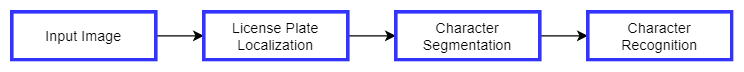
\includegraphics[scale=.55]{images/sys_block_diagram.png}
    		\caption{Sơ đồ khối của hệ thống}
    		\label{fig:sysblockdiagram}
    	\end{figure}
    \textbf{Hoạt động}
\include{main/ch2_theoryofmesh}
\include{main/ch3_design}
\chapter{Quá trình hiện thực}
Từ giới hạn đề tài và cơ sở lý thuyết, ta chia quá trình hiện thực thành ba phần tương đối độc lập:
\begin{itemize}
    \item Hiện thực quá trình xác định vùng biển số và vùng ký tự.
    \item Hiện thực BNN nhận dạng các ký tự đã tìm được.
    \item Tạo overlay gia tốc cho quá trình xác định vùng biển số và vùng ký tự.
\end{itemize}

\section{LP Detection and Character Segmentation}
\section{Character Regcongition}
\section{Tạo overlay gia tốc cho quá trình xác định vùng biển số và ký tự}
Từ quá trình hiện thực tim vùng biển số và ký tự ta có thể thấy, hàm gắn nhãn đối tượng được sử dụng thường xuyên. Vì vậy, để khai thác tính tái sử dụng cho overlay, nhóm quyết định chọn hàm gắn nhãn đối tượng cho việc tạo overlay.

    \subsection{Hàm gắn nhãn đối tượng}
    \textbf{Về hàm cần gia tốc: skimage.measure.label}
    
    Hàm skimage.measure.label(input[, neighbors, …]) là hàm ngắn nhãn những vùng được liên kết với nhau trong một mảng số nguyên (ví dụ: ảnh nhị phân).
    
    Chi tiết về hàm xem tại: \url{https://scikit-image.org/docs/dev/api/skimage.measure.html#skimage.measure.label}
    
    \textbf{Chức năng hàm gia tốc hw\_label\_accel}
    
    Protype của hàm:
    hw\_label\_accel(axis\_t *src, axis\_t *dst, int rows, int cols).
    
    Trong đồ án này, đầu vào của hàm là một ảnh nhị phân (ma trận 2 chiều) nên chức năng của hàm trở nên đơn giản hơn so với hàm skimage.measure.label() về:
    \begin{itemize}
        \item input: input của hw\_label\_accel (src) là ảnh nhị phân hay một mảng các giá trị nguyên trong khi input của skimage.measure.label() có thể là ma trận 2 hay 3 chiều.
        \item neighbors: Một điểm trong input của hw\_label\_accel có số hàng xóm tối đa luôn là 8 thay vì có thể là 4 hoặc 8.
        \item background: Nền trong input của hw\_label\_accel luôn có giá trị là 0 thay vì có thể lựa chọn.
        \item Returns: Giá trị trả về của hw\_label\_accel (dst)là một mảng số nguyên hay một ảnh xám. Nó đồng nhất với giá trị trả về của skimage.measure.label (labels).
    \end{itemize}
    
    \subsection{Giải thuật của hàm gia tốc}
    
    Hình \ref{fig:overlayalgorithmflow} thể hiện giải thuật cho hàm hw\_label\_accel. Trong đó:
    \begin{itemize}
        \item Hàm ismarked(src[i]) trả về TRUE nếu điểm i đã được gắn nhãn và FALSE nếu chưa.
        \item Hàm mark(src[idx]) sẽ gắn nhãn cho giá trị tại điểm idx. Giá trị của nhãn phụ thuộc vào số lượng nhãn đã được sử dụng.
        \item Hàm FB\_neighbors(i) trả về những điểm kế của i mà tại đó src[i] chưa được gắn nhãn.
    \end{itemize}
    Kết thúc hàm ta sẽ thu đươc src là output cần tìn. Ta cần đầy src ra ngõ ra.
    \begin{figure}[htp]
    	\centering
     	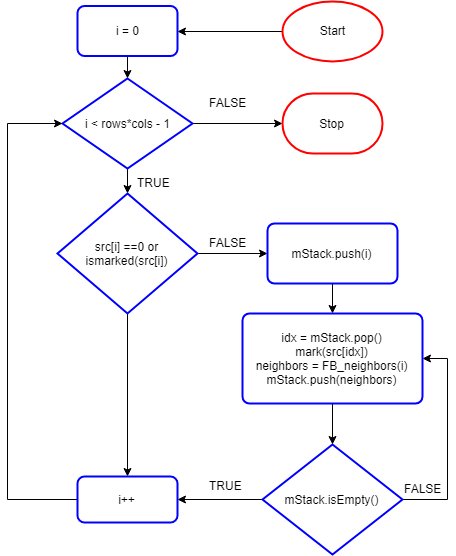
\includegraphics[scale=.8]{images/overlay_algo_flow.png}
    	\caption{Giải thuật cho hàm hw\_label\_accel}
    	\label{fig:overlayalgorithmflow}
    \end{figure}
    
    \subsection{Hiện thực hàm hw\_label\_accel bằng Vivado HLS}
    
\chapter{Kịch bản thử nghiệm} \label{chap:experiment}
    \section{Mục tiêu của thử nghiệm}
    \section{Quá trình thử nghiệm}
        \subsection{Kịch bản I:}
\chapter{Kết luận}\label{chap:conclude}
    \section{Đánh giá kết quả}
    	\subsection{Thành quả đạt được}
    
        \subsection{Một số hạn chế}
    \section{Hướng phát triển}
%\include{main/experiment}
%\include{main/conclusion}


%%%%%%%%%%%%%%%%%%%%%%%%%%%%%%%%%%%%%%%%%%%%%%
%%%%% TAIL: Bibliography, Appendix, CV
%%%%%%%%%%%%%%%%%%%%%%%%%%%%%%%%%%%%%%%%%%%%%%
\appendix
\chapter{Hướng dẫn thực thi ứng dụng}\label{guide}
\backmatter
\cleardoublepage
\renewcommand{\bibname}{Tài liệu tham khảo}
\begin{thebibliography}{80}
%[1]
\bibitem{zynq}
Xilinx Zynq là gì?
\\\texttt{\url{https://www.xilinx.com/products/silicon-devices/soc/zynq-7000.html}}

\end{thebibliography}
\addcontentsline{toc}{chapter}{Tài liệu tham khảo}


% Add your glossary here
% Add your index here
% Photographic credits (list of pictures&images that have been used with names of the person holding the copyright for them)
%\include{tail/cv}

\end{document}
\grid
